\newchapter{phasePropagation}{Phase Propagation}

This is the introductory text.

\newsection{phaseJitDefs}{Definitions of Different Phase Statistics}

Definitions of different types of phase jitter.


\newsection{origJitter}{Characteristics of Uncorrected Phase Jitter}

Injector feedbacks etc.

\newsection{r56}{First Order Energy Dependencies}

\subsection{Correlation between Phase and Energy}
\label{ss:corrPhaseEnergy}

energy jitter

Upstream AND downstream


\subsection{R56}
\label{ss:r56Equations}

Assuming energy is the only source of differences between the upstream and downstream phase, the downstream phase, \(\phi_d\), can be expressed in terms of the optics transfer matrix coefficient \(R_{56}\) (Section~\ref{s:opticsIntro}) as follows:
\begin{equation}
\phi_d = \phi_u + R_{56}\frac{\Delta p}{p}
\label{e:r56PhasEq}
\end{equation}

Where \(\phi_u\) is the upstream phase, \(\Delta p / p\) is the relative energy offset and \(R_{56}\) is the R56 value between the upstream and downstream phase monitors, defined by the machine optics. R56 defines the phase shift between two points in the lattice resulting from a beam energy offset. The units of R56 in the equation above are 12~GHz radians per unit relative energy offset (\(\Delta p/p = 1\)). MADX uses units of metres and this value is what will be referred to in this chapter. To obtain the R56 value to use in the equation above the MADX value must be multiplied by the conversion factor \(2\pi/0.025\), where 0.025~m is the 12~GHz wavelength.

In terms of jitters Equation~\ref{e:r56PhasEq} becomes:
\begin{equation}
\sigma_d = \sqrt{\sigma_u^2 + R_{56}^2\sigma_{p}^2 + 2R_{56}\rho_{up}\sigma_{u}\sigma_{p}}
\label{e:r56JitEq}
\end{equation}
Where \(\sigma_d\) is the downstream phase jitter, \(\sigma_u\) is the upstream phase jitter, \(\sigma_p\) is the relative energy jitter and \(\rho_{up}\) is the correlation between the upstream phase and the energy. This follows from the result of adding correlated variances. Clearly, any non-zero R56 between the upstream and downstream phase monitors introduces an additional energy component to the downstream phase that increases the downstream phase jitter.

The effect of R56 on the upstream-downstream phase correlation, \(\rho_{ud}\), can also be defined starting from the definition of the correlation coefficient:
\begin{equation}
\rho_{ud} = \frac{\mathrm{cov}\left[\phi_u,\phi_d\right]}{\sigma_u\sigma_d}
\label{e:r56CorrDef1}
\end{equation}
Where \(\mathrm{cov}\left[\phi_u,\phi_d\right]\) is the covariance between the upstream and downstream phase, given by:
\begin{equation}
 \mathrm{cov}\left[\phi_u,\phi_d\right] = \frac{1}{N} \sum_{i=1}^{N}\phi_{ui}\phi_{di}
\label{e:r56CorrDef2}
\end{equation} 
By inserting the definition of the downstream phase from Equation~\ref{e:r56PhasEq} and separating the terms in the sum this becomes:
\begin{equation}
\mathrm{cov}\left[\phi_u,\phi_d\right] = \frac{1}{N} \sum_{i=1}^{N}\phi_{ui}^{2} + R_{56}\frac{1}{N} \sum_{i=1}^{N}\phi_{ui}\frac{\Delta p}{p}
\label{e:r56CorrDef3}
\end{equation}
The first term is now the variance of the upstream phase, \(\sigma_u^2\), and the second term is \(R_{56}\) multiplied by the covariance between the upstream phase and the energy, \(\mathrm{cov}\left[\phi_u,\frac{\Delta p}{p}\right]\), which can be expressed in terms of the correlation between the upstream phase and the energy, \(\rho_{up}\):
\begin{equation}
\mathrm{cov}\left[\phi_u,\frac{\Delta p}{p}\right] = \rho_{up}\sigma_u\sigma_{p}
\label{e:r56CorrDef4}
\end{equation}
Therefore, Equation~\ref{e:r56CorrDef3} becomes:
\begin{equation}
\mathrm{cov}\left[\phi_u,\phi_d\right] = \sigma_u^2 + R_{56}\rho_{up}\sigma_u\sigma_p
\label{e:r56CorrDef5}
\end{equation}
Finally, substituting Equations~\ref{e:r56JitEq}~and~\ref{e:r56CorrDef5} into Equation~\ref{e:r56CorrDef1} gives:
\begin{equation}
\rho_{ud} = \frac{\sigma_u + R_{56}\rho_{up}\sigma_p}{\sqrt{\sigma_u^2 + R_{56}^2\sigma_{p}^2 + 2R_{56}\rho_{up}\sigma_{u}\sigma_{p}}}
\label{e:r56CorrDefFinal}
\end{equation}

Considering that in this model the only difference between the upstream and downstream phase results from the R56, it is perhaps obvious that the best conditions for the PFF correction are obtained when the R56 coefficient between the upstream and downstream phase monitors is zero. In these conditions \(\sigma_d = \sigma_u\) and \(\rho_{ud} = 1\). This can be more formally defined by using the expression for the theoretical corrected downstream phase jitter when using the optimal gain factor as derived in Section~\ref{ss:theoryJitter}:
\begin{equation}
\sigma_{PFF} = \sigma_d\sqrt{1-\rho_{ud}^2}
\end{equation}
All these quantities have been derived above and inserting them in to this equation gives the following expression for the corrected downstream phase jitter in terms of the R56:
\begin{equation}
\sigma_{PFF} = \left|R_{56}\right|\sigma_p\sqrt{1-\rho_{up}^2}
\label{e:r56PFFJit}
\end{equation}
As expected the achievable corrected downstream phase jitter is minimised when \(R_{56}~=~0\). Note that this equation does not take in to account the effects of the phase monitor resolution, which in reality limits the minimum achievable downstream phase jitter to \(\sigma_{PFF}=0.2^\circ\) ([TODO:Section ref]). 

In principle the beam conditions for the PFF correction could also be improved by reducing the relative energy jitter (\(\sigma_p\)) or by increasing the upstream phase-energy correlation (\(\rho_{up}\)). Reducing the relative energy jitter decreases the additional phase jitter created by non-zero R56. Increasing the upstream phase-energy correlation (\(\rho_{up}\)) reduces the effect that non-zero R56 has on the upstream-downstream phase correlation (\(\rho_{ud}\)). For example, if \(\rho_{up}=1\) the source of all upstream phase jitter is energy jitter. In that case although non-zero R56 would further increase the downstream phase jitter, the additional jitter would be well correlated with the upstream phase and the upstream-downstream phase correlation would not be affected. In practice \(\sigma_p\) and \(\rho_{up}\) are defined by the CTF3 injector and can not be varied with a great degree of flexibility, so having zero R56 is the only way to obtain ideal conditions for the PFF correction. High upstream phase-energy correlations can be created at CTF3 but not without greatly amplifying the upstream phase jitter, which causes issues for the PFF system due to its limited correction range (Section~\ref{s:pffNovelSetups}).

An interesting side note of Equations~\ref{e:r56JitEq}~and~\ref{e:r56PFFJit} is that the best beam conditions for the PFF correction are not given by minimising the initial downstream phase jitter in the case where the upstream phase-energy correlation, \(\rho_{up}\), is non-zero. As seen in the previous section in normal conditions there is a small correlation between the upstream phase and the energy at CTF3, typically around \(\rho_{up}=0.2\). In these conditions the downstream phase jitter can in theory be reduced to below the level of the upstream phase jitter by using a negative R56 to remove the energy component in the downstream phase. Differentiating Equation~\ref{e:r56JitEq} gives the minimum downstream phase jitter to be obtained when \(R_{56} = -\rho_{up}\sigma_u/\sigma_p\). However, using this \(R_{56}\) value would degrade the upstream-downstream phase correlation and increase the achievable corrected downstream jitter, which is always minimised when \(R_{56} = 0\) as in Equation~\ref{e:r56PFFJit}. This is significant for the \(R_{56}\) optimisation attempts presented later in this chapter, as it must always be kept in mind that the goal is to maximise the upstream-downstream phase correlation rather than to create the most stable downstream phase (with the PFF system off).

\subsection{Effect of R56 in TL2}
\label{ss:r56TL2Effect}

Unfortunately, it was not possible to find optics for the TL2 chicane that met all the PFF requirements and thus an R56 in the chicane of close to -0.2~m had to be accepeted (Section~\ref{ss:pffMatched}). All other lines at CTF3 nominally have zero R56 [REF], and therefore don't introduce additional phase jitter via energy, at least to first order and to within the accuracy of the CTF3 MADX model. The overall R56 between the upstream phase monitors (in the CT line) and the downstream phase monitors (in the TBL line, labelled CB, after the TL2 chicane) is therefore -0.2~m also. Whether this can explain the low upstream-downstream phase correlation and high downstream phase jitter seen in Section~\ref{s:origJitter}, as well as what residual R56 between the two monitors can be tolerated to be able to achieve CLIC-level phase stability at CTF3, is discussed in this section.

Equations~\ref{e:r56JitEq}~and~\ref{e:r56CorrDefFinal} can be used to estimate the downstream phase jitter and upstream-downstream phase correlation in the conditions at CTF3. Typical values for the various parameters in the equations have already been presented in previous sections, and these values are summarised in Table~\ref{t:r56Params}. The value \(R_{56}\simeq -0.2\) was obtained in Section~\ref{ss:pffMatched} as previously mentioned, the value \(\sigma_u\simeq0.8^\circ\) in Section~\ref{s:origJitter} and the values \(\rho_{up}\simeq 0.2\) and \(\sigma_p\simeq 0.001\) in Section~\ref{ss:corrPhaseEnergy}.

\begin{table}
  \begin{center}
    \begin{tabular}{| c c |}
	   \hline
       Parameter & Value \\ \hline
       \(R_{56}\) & -0.2~m \\
       \(\sigma_u\) & \(0.8^\circ\) \\
       \(\rho_{up}\) & 0.2 \\
       \(\sigma_{p}\) & 0.001 \\ \hline
    \end{tabular}
    \caption{Typical upstream phase and energy conditions at CTF3.}
  	\label{t:r56Params}
  \end{center}
\end{table}

With these parameter values the residual R56 of -0.2~m reduces the upstream-downstream phase correlation to below 10\% [TODO: 45\% on the other side of the crest, and there is ambiguity], and amplifies the downstream phase jitter to above 3~degrees. R56 transforming energy jitter in to downstream phase jitter therefore explains the low upstream-downstream phase correlation and high downstream phase jitter seen in Section~\ref{s:origJitter}. In order to increase the upstream-downstream phase correlation to 97\% and reduce the downstream jitter to 0.8~degrees (the conditions needed to achieve 0.2~degrees corrected downstream phase jitter at CTF3, see Section~\ref{s:pffEquations}) the R56 between the upstream and downstream phase monitors must be removed.

Figure~\ref{f:jitVsR56}~and~\ref{f:corrVsR56} show the expected downstream phase jitter and upstream-downstream phase correlation for residual R56 values from -0.2 to +0.2~m between the upstream and downstream phase monitors again using the equations derived in the previous section. The horizontal black line in each figure marks the requirements needed to reduce an initial upstream phase jitter of 0.8 degrees to the CLIC target of 0.2 degrees. The red line, "corrected", in Figure~\ref{f:jitVsR56} shows the theoretical corrected downstream phase jitter using the PFF correction across the range of R56 values. Note the slight asymmetry in the phase jitter and correlation curves, which is caused by the non-zero correlation between the upstream phase and the beam energy. In order to obtain CLIC level phase stability at CTF3 the residual R56 between the upstream and downstream phase monitors must be reduced from the initial \(-0.2m\) to \(0\pm1.3~cm\).

\begin{figure}
  \centering
  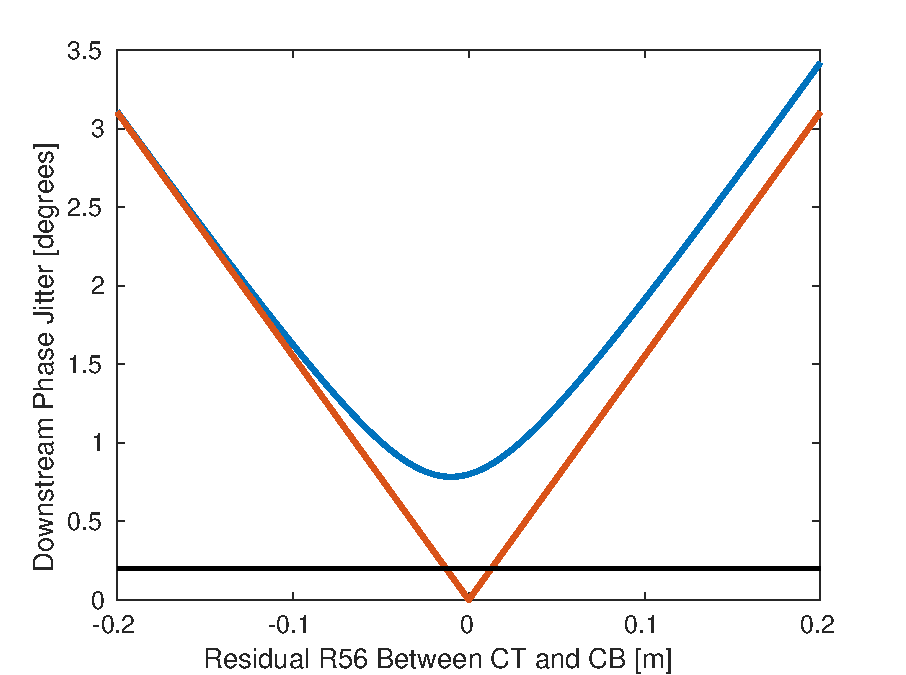
\includegraphics[width=0.9\textwidth]{Figures/propagation/jitVsR56}
  \caption{Downstream phase jitter vs. residual R56 between monitors.}
  \label{f:jitVsR56}
\end{figure}

\begin{figure}
  \centering
  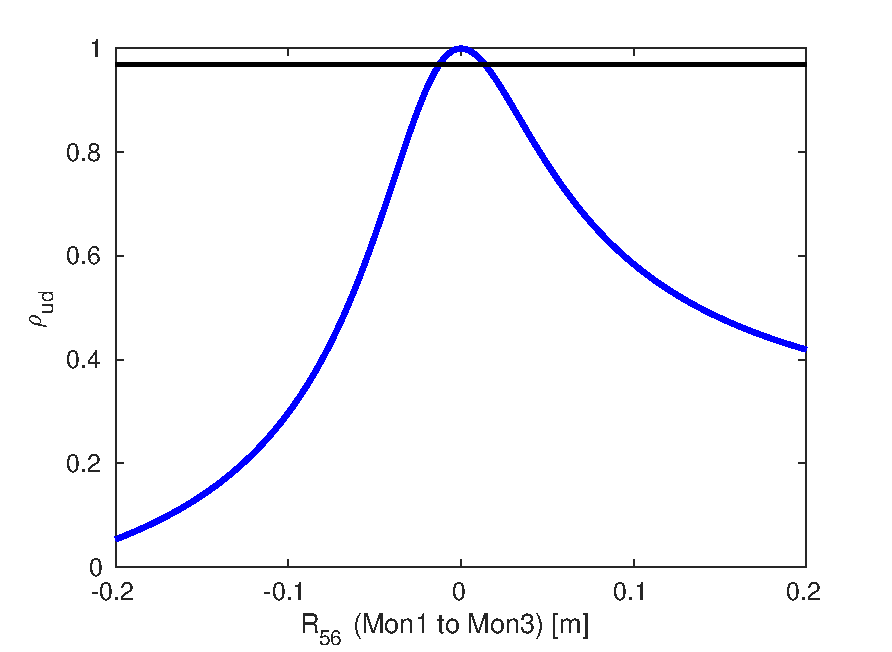
\includegraphics[width=0.9\textwidth]{Figures/propagation/corrVsR56}
  \caption{Phase correlation vs. residual R56 between monitors.}
  \label{f:corrVsR56}
\end{figure}

To interpret the results of the R56 optimisation attempts presented in the remainder of this chapter it is useful to understand how varying the correlation between the usptream phase and the energy (\(\rho_{up}\) changes the dependence of the upstream-downstream phase correlation (\(\rho_{ud}\)) on the residual R56. In particular, in Section~\ref{ss:r56ScanWithEnergy} a machine setup that increases \(\rho_{up}\) to 90\% was used. Figure~\ref{f:corrVsR56_CTENCorr} shows how \(\rho_{ud}\) varies with \(\rho_{up}\) values between 0\% and 40\% (typical of normal operation) and with the higher correlation of 90\%. With high correlations between the upstream phase and energy there is no longer a well defined peak in \(\rho_{ud}\) versus the residual R56 value. Instead there is an almost constant high upstream-downstream phase correlation with positive R56 values, and a large anti-correlation for negative R56 values (as in this case the residual R56 acts to flip the sign of the phase jitter). 

\begin{figure}
  \centering
  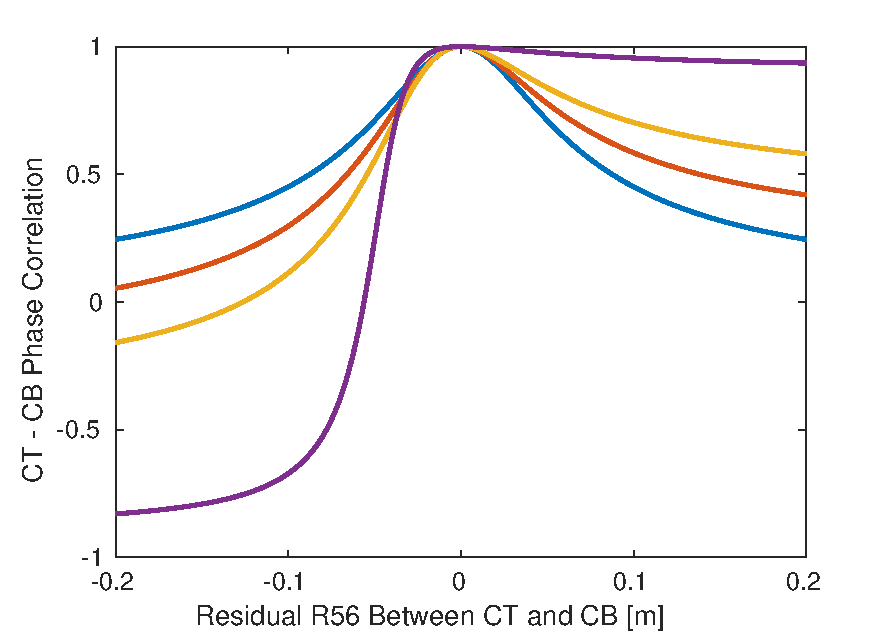
\includegraphics[width=0.9\textwidth]{Figures/propagation/corrVsR56_CTENCorr}
  \caption{Phase correlation vs. residual R56 between monitors.}
  \label{f:corrVsR56_CTENCorr}
\end{figure}

In Figure~\ref{f:jitVsR56_90ctencorr} plotting the theoretical downstream jitter with \(\rho_{up} = 0.9\) gives a clear demonstration that the best conditions for the PFF correction are always with \(R_{56} = 0\) rather than with the lowest possible initial downstream jitter, as mentioned in the previous section. In fact, as these conditions relax the requirements on the residual R56 needed to achieve high upstream-downstream phase correlations (as seen in the previous figure) it may be easier to achieve a large factor reduction in the downstream phase jitter with the PFF system with a high \(\rho_{up}\) machine setup. This has been attempted and is presented in Section~\ref{s:pffNovelSetups}.

\begin{figure}
  \centering
  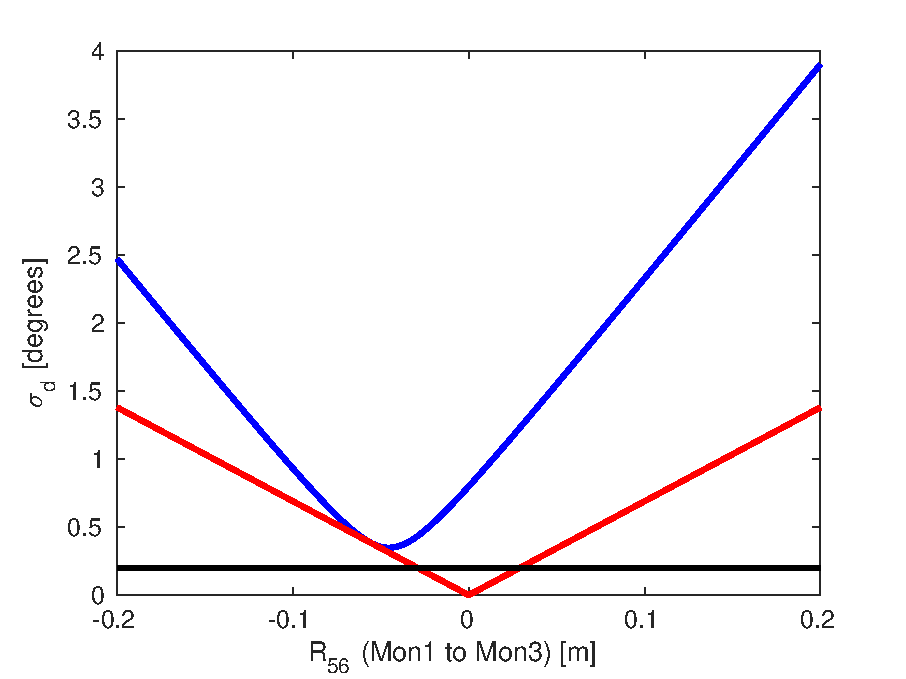
\includegraphics[width=0.9\textwidth]{Figures/propagation/jitVsR56_90ctencorr}
  \caption{Phase correlation vs. residual R56 between monitors.}
  \label{f:jitVsR56_90ctencorr}
\end{figure}

\newsection{r56Removal}{Mitigation of First Order Energy Dependence}

The discussion in the previous section proves that with a residual R56 value of -0.2~m between the upstream and downstream phase monitors it is impossible to achieve the goals of the PFF prototype at CTF3. However, due to the highly constrained optics in TL2 it has already been seen in Chapter~\ref{c:tl2Optics} that it was not possible to find optics for the PFF chicane that yield zero R56 whilst also meeting requirements for both the PFF system and transverse matching (dispersion and beta functions). The only way to create a total R56 of zero between the upstream and downstream phase monitors is therefore to add positive R56 to one of the other beam lines at CTF3 in order to compensate for the negative R56 in the TL2 chicane. 

The previous transfer line TL1, which transports the beam from the CT line (where the upstream phase monitors are installed) to the combiner ring (see Figure~\ref{f:ctfLayout}), has been used to achieve this. The layout of the TL1 transfer line is shown in Figure~\ref{f:tl1Layout}. It consists of: 4 dipoles (bending the beam horizontally) of 2 different types, 13 quadrupoles of 5 different types, 7 magnetic correctors, 1 sextupole (usually not used) and 8 BPMs (the dispersive BPM after the first dipole in TL1, labelled CT.BPI0608, is the device that has been used to determine correlations between the phase and energy in this chapter). The total length of TL1 is approximately 30~m.
[TODO: more details?]

Preliminary attempts to reduce the residual R56 between the upstream and downstream phase monitors using TL1 yielded correlations up to 60\% and reduced the downstream phase jitter to \(2^\circ\). Conditions similar to these were used for the first PFF tests (Chapter~\ref{c:earlyFFSim}) before the energy related effects discussed in this chapter were fully characterised, but in these tests only a modest reduction of 30\% in downstream phase jitter was possible due to the limitations of the phase propagation shown here. At this time only a few different optics for TL1 were available in R56 steps of 10~cm. As the total residual R56 must be reduced to the centimetre level to make a correction down to 0.2 degrees jitter theoretically possible with the PFF system, new sets of optics for TL1 were required.

\begin{landscape}
	\begin{figure}
  		\centering
  		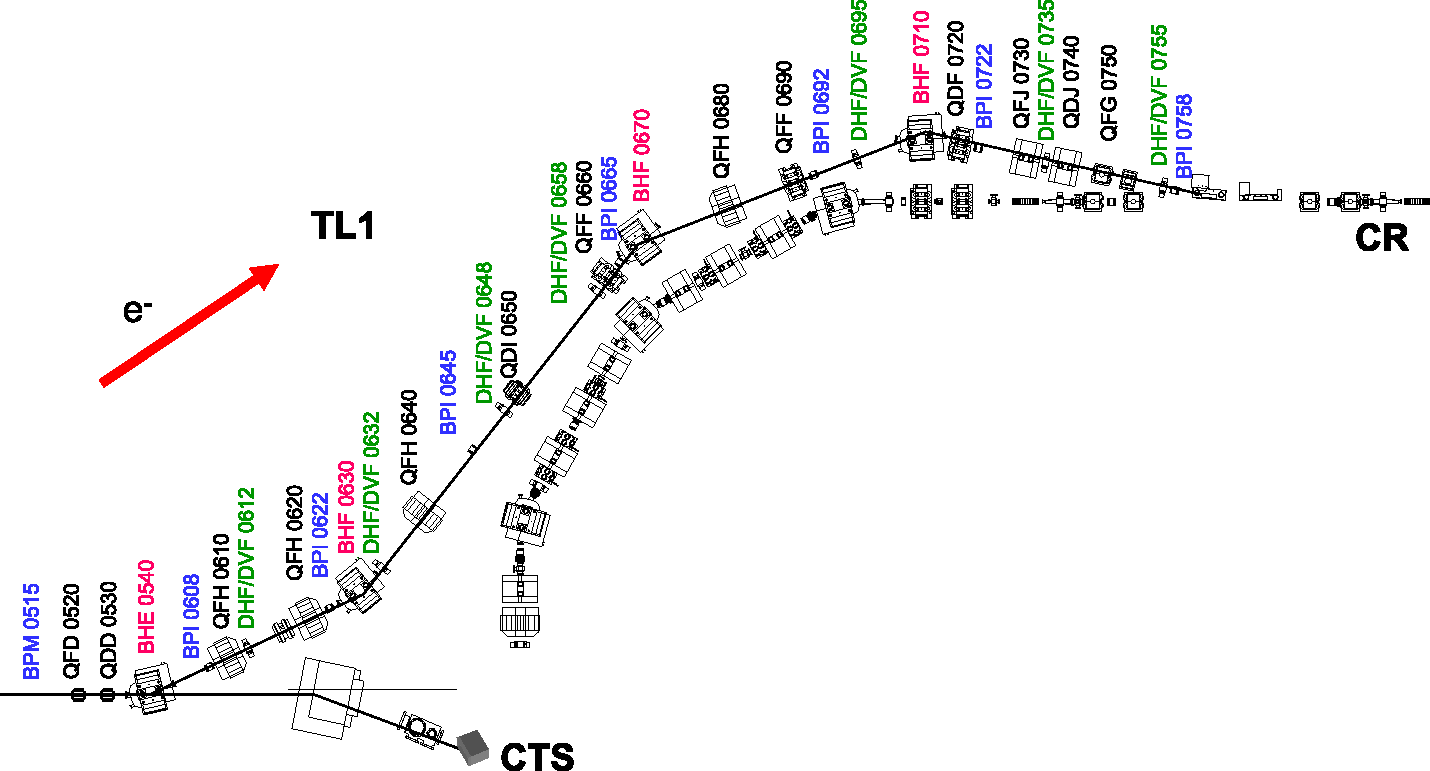
\includegraphics[height=\textwidth]{Figures/propagation/TL1}
  		\caption{TL1.}
  		\label{f:tl1Layout}
	\end{figure}
\end{landscape}
[TODO: Need a better figure]

\subsection{Matched Optics for TL1}
\label{ss:tl1Optics}

Although in theory only one set of optics with \(R_{56} = +0.2\)~m in TL1 is required to compensate for the \(R_{56} = -0.2\)~m in TL2, in practice errors in the MADX model of CTF3 plus the effect of higher order energy dependencies (see Section~\ref{s:t566}) means it is not possible to know precisely what the optimal R56 to set in TL1 will be, and it is also possible that this value will vary with time. To determine the optimal value of R56 to set it is also useful to scan the R56 value in TL1 across a wide range of values and then fit the maximum resulting upstream-downstream phase correlation.

To allow this, MADX has been used to match optics for TL1 with R56 values ranging from -0.3~m to +0.6~m in steps of 0.5~cm (a total of 181 sets of optics). The optimal R56 value should always be guaranteed to be in this range, and the step size of 0.5~cm allows the residual R56 to be zeroed to within one centimetre as derived to be necessary in Section~\ref{ss:r56TL2Effect}. As well as the different R56 values, each set of optics must maintain the same initial and final conditions, so that the injection of the beam in to the combiner ring is not affected. Values for the beta functions, alphas and dispersion at the start of TL1 and at the combiner ring injection are summarised in Table~\ref{t:tl1MatchParams}. As well as the initial and final conditions, the maximum beta functions and dispersion in TL1 are constrained to ensure a reasonable beam size throughout the line --- the horizontal and vertical beta function is limited to a maximum of 35~m, and the horizontal dispersion to a maximum absolute value of 1.25~m. Around the septum used for injection in to the combiner ring the horizontal beta function is further limited to a maximum of 10~m. The strengths of the 13 quadrupoles in TL1 are varied to meet all these constraints.

\begin{table}
  \begin{center}
    \begin{tabular}{| c c c |}
	   \hline
       Parameter & TL1 Injection & CR Injection \\ \hline
       \(\beta_x\) & 8.81~m & 4.08~m \\
       \(\beta_y\) & 13.94~m & 5.41~m \\
       \(\alpha_x\) & -0.74 & -0.31 \\
       \(\alpha_y\) & -0.45 & -0.21 \\ 
       \(D_x\) & 0~m & -0.03~m \\ 
       \(D_{px}\) & 0 & 0.02 \\ \hline
    \end{tabular}
    \caption{Initial and final conditions for optics matching in TL1.}
  	\label{t:tl1MatchParams}
  \end{center}
\end{table}

Figures~\ref{f:r56MatchedVsTarget} shows the matched R56 value in TL1 across the range of targeted values. Each matched R56 value is within 10 microns of the desired result. Figure~\ref{f:CTQFG0750} then shows an example of how the strength of one of the quadrupoles must be varied in order to achieve each R56 value. If the dependence of each quadrupole strength on the R56 value was continuous the relationship could be fitted to create a set of tuning knobs to allow R56 to be set to any arbitrary value in TL1. However, as seen in the figure there are many discontinuities. The quadrupole strengths for each set of optics are therefore saved to a lookup table, with a MatLab function created to read the table and set the quadrupole currents in the machine appropriate for the specified R56 value. As already mentioned 0.5~cm precision in R56 should be adequate for the PFF requirements, but the discontinuities mean new optics would have to be matched if optics with an R56 value not included in the discrete set used here were required.

\begin{figure}
  \centering
  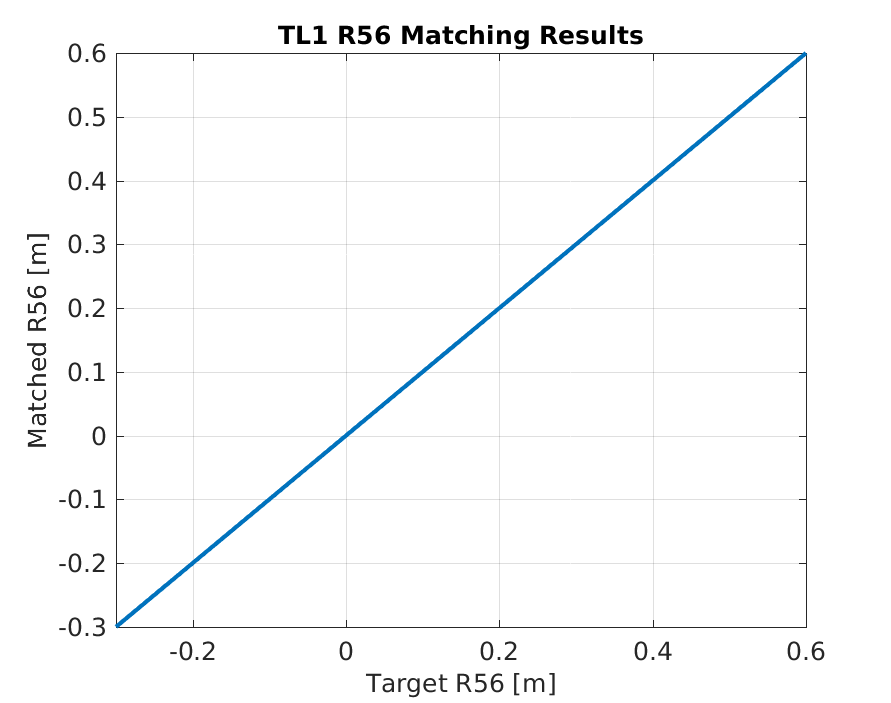
\includegraphics[width=0.9\textwidth]{Figures/propagation/r56MatchedVsTarget}
  \caption{Matched R56 values for TL1.}
  \label{f:r56MatchedVsTarget}
\end{figure}

\begin{figure}
  \centering
  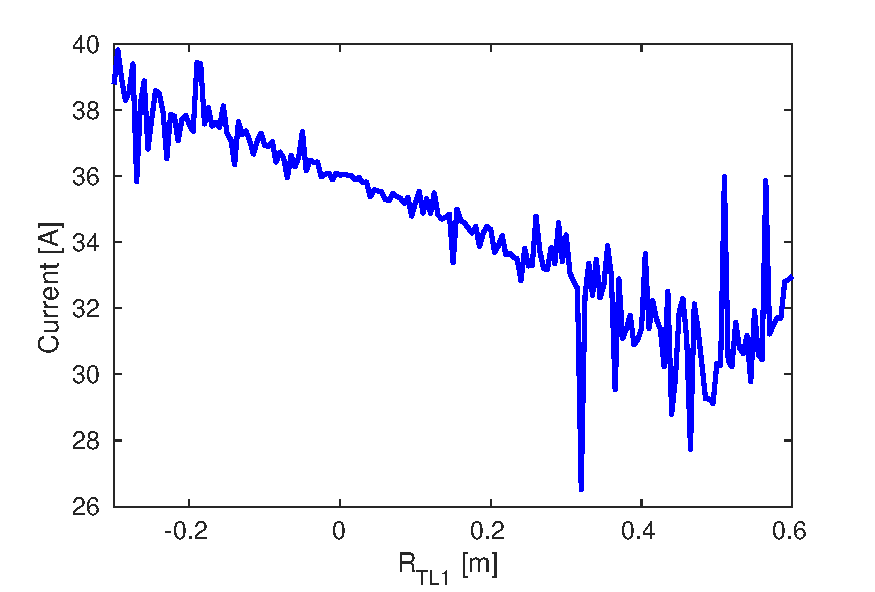
\includegraphics[width=0.9\textwidth]{Figures/propagation/CTQFG0750}
  \caption{Current vs. R56 for the CT.QFG0750 quadrupole in TL1.}
  \label{f:CTQFG0750}
\end{figure}

For reference Figures~\ref{f:tl1BETX}~\ref{f:tl1BETY}~and~\ref{f:tl1DX} show how the horizontal and vertical beta functions and horizontal dispersion changes in TL1 for each set of optics. For all R56 values each parameter converges to the same value at the start and end of TL1, as needed to ensure that changing the R56 does not impact injection in to the combiner ring. The maximum horizontal and vertical beta functions in TL1 roughly increase with the set R56 value, but in all cases are kept below the set limit of 35~m in the matching procedure. The dispersion pattern in TL1 also changes with the set R56 value, though in most cases the maximum absolute dispersion is around 1~m and only the location of the peak dispersion along the line changes. Again, for each set of optics the maximum absolute dispersion is limited within the set constraint of 1.25~m. 

\begin{figure}
  \centering
  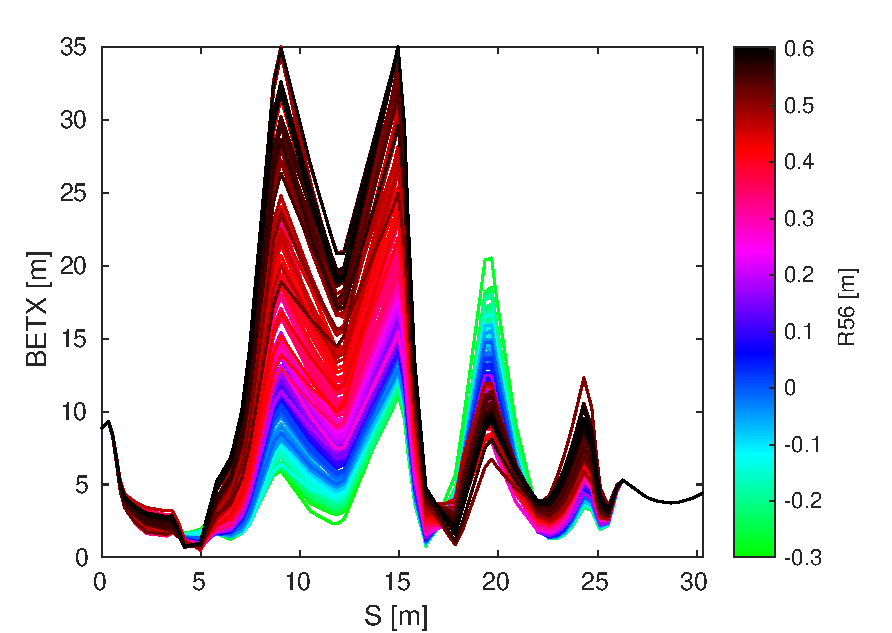
\includegraphics[width=0.9\textwidth]{Figures/propagation/BETX}
  \caption{Horizontal beta in TL1 for all R56 optics.}
  \label{f:tl1BETX}
\end{figure}

\begin{figure}
  \centering
  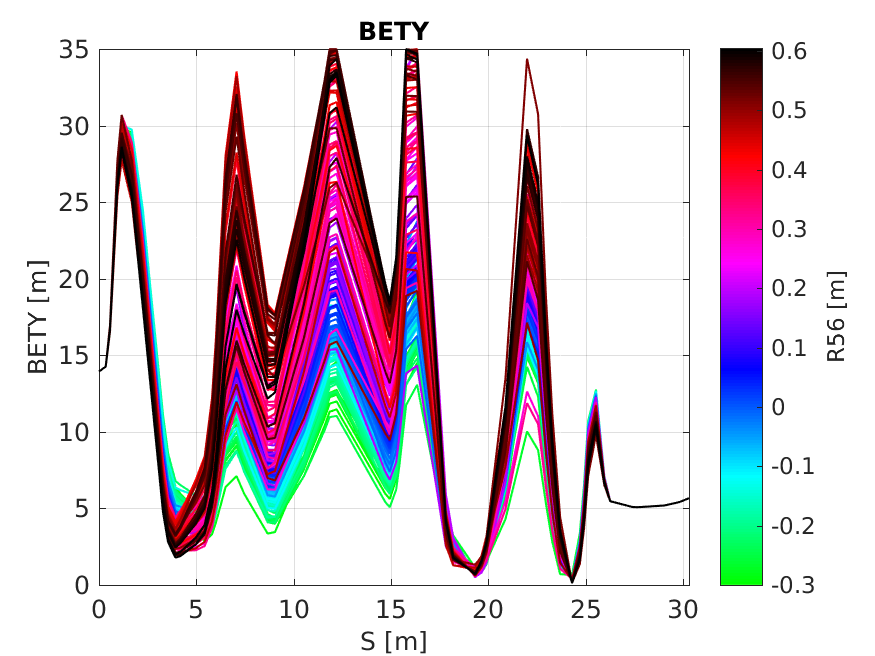
\includegraphics[width=0.9\textwidth]{Figures/propagation/BETY}
  \caption{Vertical beta in TL1 for all R56 optics.}
  \label{f:tl1BETY}
\end{figure}

\begin{figure}
  \centering
  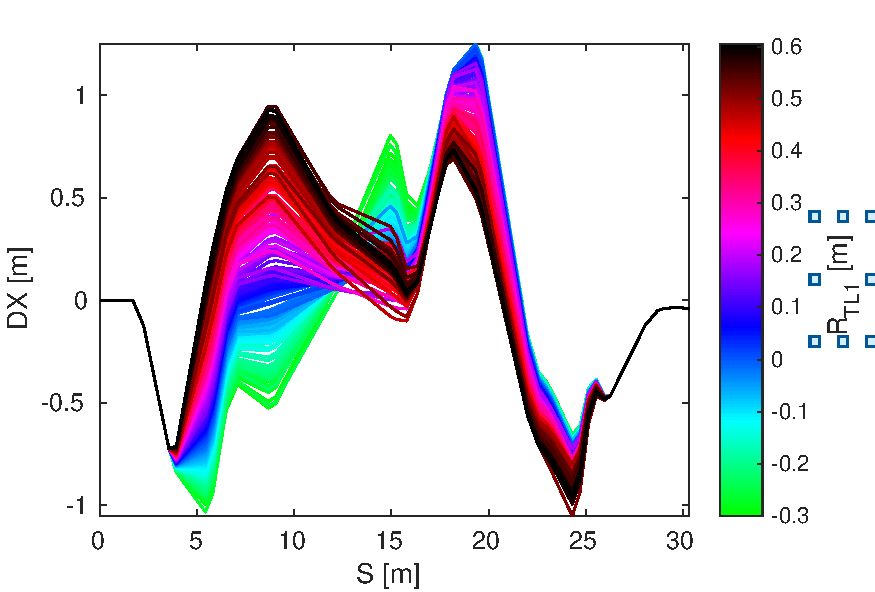
\includegraphics[width=0.9\textwidth]{Figures/propagation/DX}
  \caption{Dispersion in TL1 for all R56 optics.}
  \label{f:tl1DX}
\end{figure}

Commissioning of the new TL1 optics in CTF3 was straightforward and in general they can be set with the quadrupole strengths at their nominal matched values without causing issues for the beam quality. At the extremities of the range of optics (close to R56 = -0.1~m and R56 = +0.6~m) some slight beam losses do begin to occur, but this is not a problem for PFF operation where the required R56 is only 0.2~m. However, for each set of optics the magnetic correctors in TL1 may need to be changed to recover the nominal beam orbit, thus taking in to account slight misalignments in elements along the line. [TODO: could expand this] 

\subsection{Scans of R56 in TL1}
\label{ss:r56Scans}

The sets of matched optics from the previous section can be used to perform scans of the R56 value in TL1 to observe how the downstream phase is affected. Scans of this type must be performed prior to all PFF data taking periods in order to optimise the beam conditions (maximise the upstream-downstream phase correlation) for the correction. More recently scans of R56 in TL1 have been performed whilst varying the beam energy, which produces cleaner results and highlights additional factors that must be taken in to account during the optimisation process, as will be shown in Section~\ref{s:t566}. 

As a starting point the simplest case, where only the TL1 optics is changed during the scan and all other parameters in the machine are left unchanged, is presented in this section. This also highlights some of the difficulties in maintaining beam conditions at CTF3, which is discussed further in Section~\ref{s:t566} and extensively in the context of the PFF correction in Section~\ref{s:longPFF}. Figures~\ref{f:r56Scan_meanPhaseJit}~and~\ref{f:r56Scan_correlation} show one example of an R56 scan performed across the full range of available optics -- from -0.1~m R56 in TL1 to +0.6~m. The R56 is incremented by 2.5~cm between datasets, to give a total of 29 R56 points in the scan, with the whole scan taking approximately one and a half hours to complete. With the knowledge gained from measurements of this type it is no longer necessary to scan the R56 across the full range to determine the ideal value, thus the optimisation of the phase propagation for PFF attempts can now be achieved on much shorter time scales.

\subsubsection{Mean Phase}

Figure~\ref{f:r56Scan_meanPhaseJit} shows the mean phase jitter during the scan both upstream and downstream. Although the noise in the measurement is quite large, the downstream phase jitter is reduced from above 2.5 degrees with zero R56 in TL1, to below 1 degree and close to the level of the upstream phase jitter by adding positive R56 in TL1. The optimal R56 value is approximately 0.175~m, in close agreement with expectations considering the -0.2~m R56 in TL2. The upstream-downstream phase correlation, in Figure~\ref{f:r56Scan_correlation}, is also maximised at this point, from an initial correlation of 20\% with zero R56 to up to 80\%.

\begin{figure}
  \centering
  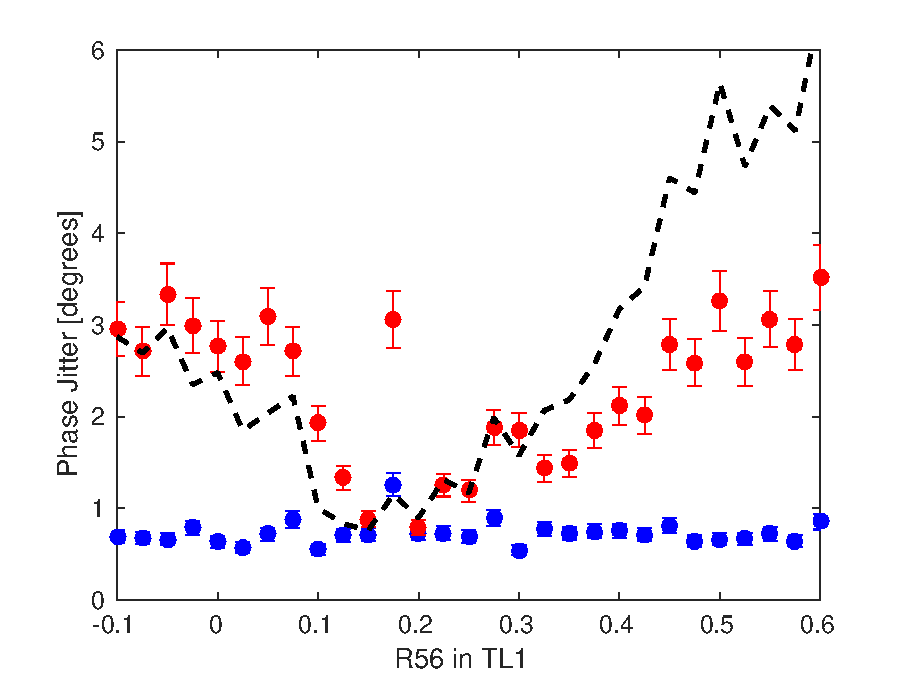
\includegraphics[width=0.9\textwidth]{Figures/propagation/r56Scan_meanPhaseJit}
  \caption{Phase jitter during scan of R56 in TL1. [TODO: Could add simulated line, agreement pretty good for R56>0 in jitter but bad R56<0. Correlation not great either]}
  \label{f:r56Scan_meanPhaseJit}
\end{figure}

\begin{figure}
  \centering
  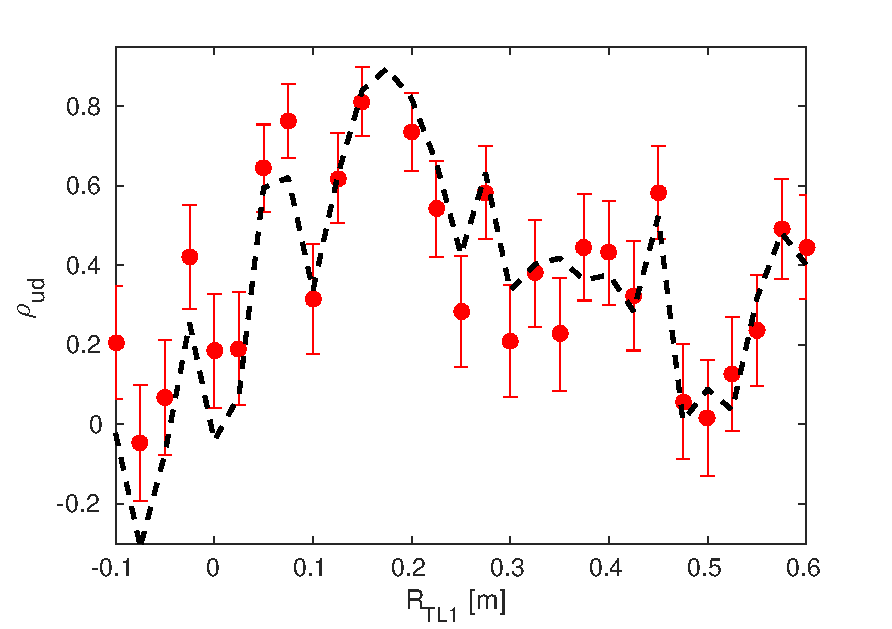
\includegraphics[width=0.9\textwidth]{Figures/propagation/r56Scan_correlation}
  \caption{Correlation during scan of R56 in TL1. Simulation is simulation-0.2}
  \label{f:r56Scan_correlation}
\end{figure}

As the upstream phase monitors are prior to TL1, changing the TL1 optics has no effect on the upstream phase jitter. All differences in the upstream phase jitter between datasets are caused by drifts in the CTF3 injector, typically changes in either klystron phases or beam current. Although the overall stability of the upstream phase jitter during this scan is good, it does vary between 0.5~degrees and 1.2~degrees. In addition to the upstream phase there are also differences in the relative energy jitter and upstream phase-energy correlation during the scan, as seen in Figure~\ref{f:r56Scan_upstreamParams}. The relative beam energy jitter varies between \(0.4\times10^{-3}\) and \(1.0\times10^{-3}\) and the upstream phase-energy correlation between -0.5 and +0.5. All these parameters influence the downstream phase, as per the equations in Section~\ref{ss:r56Equations}.

The differences in the upstream phase and energy conditions between datasets partially explains the apparent spread of the data points away from the expected clean distribution. The black ``simulation'' lines in Figures~\ref{f:r56Scan_meanPhaseJit}~and~\ref{f:r56Scan_correlation} represent the expected downstream phase jitter and upstream-downstream phase correlation at each point in the scan given the upstream phase jitter, relative energy jitter and upstream phase-energy correlation at that time (using Equations~\ref{e:r56JitEq}~and~\ref{e:r56CorrDefFinal}). The correlation simulation in Figure~\ref{f:r56Scan_correlation} has been scaled so that the peak value is in agreement with the data, at 0.8. The majority of the data points follow the scaled simulated distribution, with several remaining outliers. For the downstream phase jitter (which uses the simulated result directly with no scaling) the agreement with the simulation is good for R56 values above 0.15~m. However, below 0.15~m the actual phase jitter seen in the scan is much larger than the simulation. One possible explanation for this is that the downstream beam current stability is up to a factor 3 worse for these points (bottom plot in Figure~\ref{f:r56Scan_upstreamParams}). Small beam losses between the monitors can induce additional jitter in the measured phase that are not characterised by the R56.

\begin{figure}
  \centering
  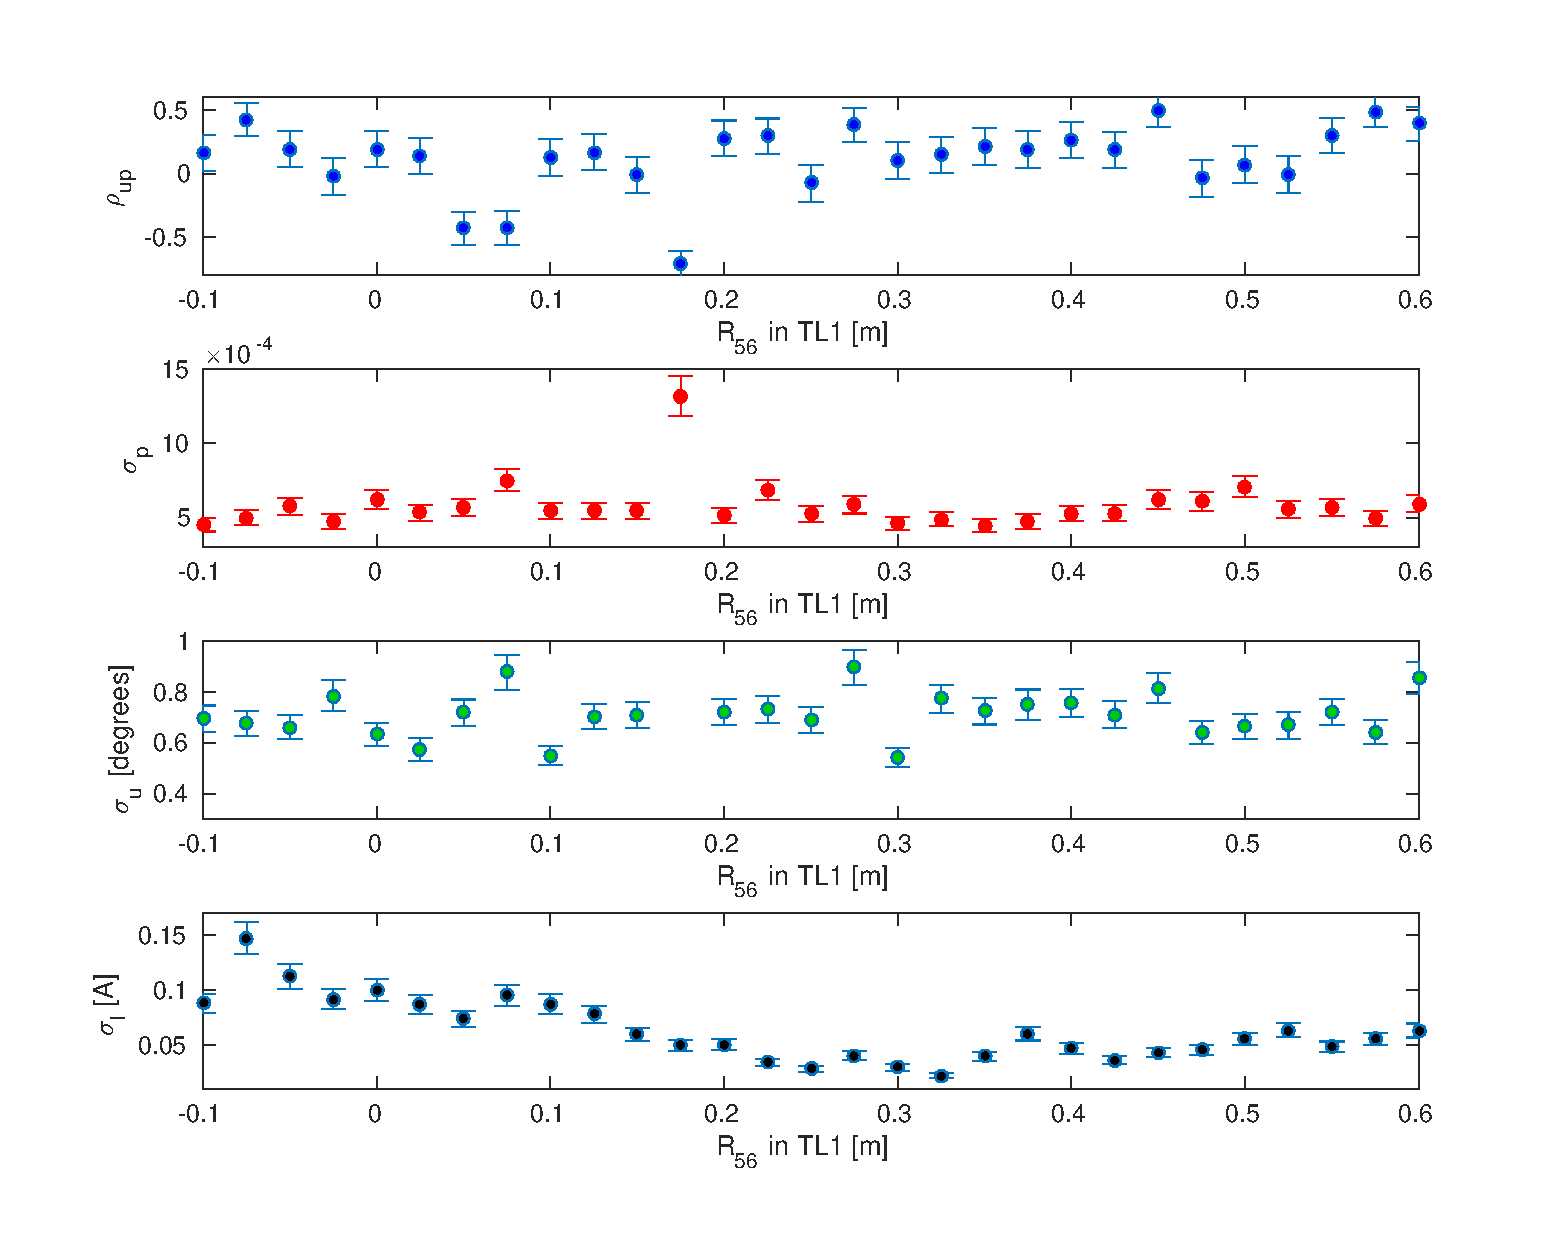
\includegraphics[width=0.9\textwidth]{Figures/propagation/r56Scan_upstreamParams}
  \caption{Upstream and downstream beam conditions during the R56 scan.}
  \label{f:r56Scan_upstreamParams}
\end{figure}

\subsubsection{Phase Along the Pulse}

As well as the mean phase it is interesting to look at the effect of varying the R56 on the phase along the pulse. Figure~\ref{f:r56Scan_meanPhaseAlong} shows the mean phase along the pulse for each R56 setting in TL1 during the scan. Any difference in the mean (rather than the jitter) along the pulse with the R56 value should originate from static energy variations along the pulse. If the energy along the pulse was constant changing the R56 would only affect the phase jitter and would not change the mean pulse shape. The clear change in certain features along the pulse in the downstream phase is therefore an indication of energy variations in these regions. Perhaps the best example of this is the oscillation around a time of 800~ns, where the phase is flat close to the optimal R56 value of 0.175~m but swings upwards when a negative R56 in TL1 is used or downards for R56 values above 0.175~m.

\begin{figure}
  \centering
  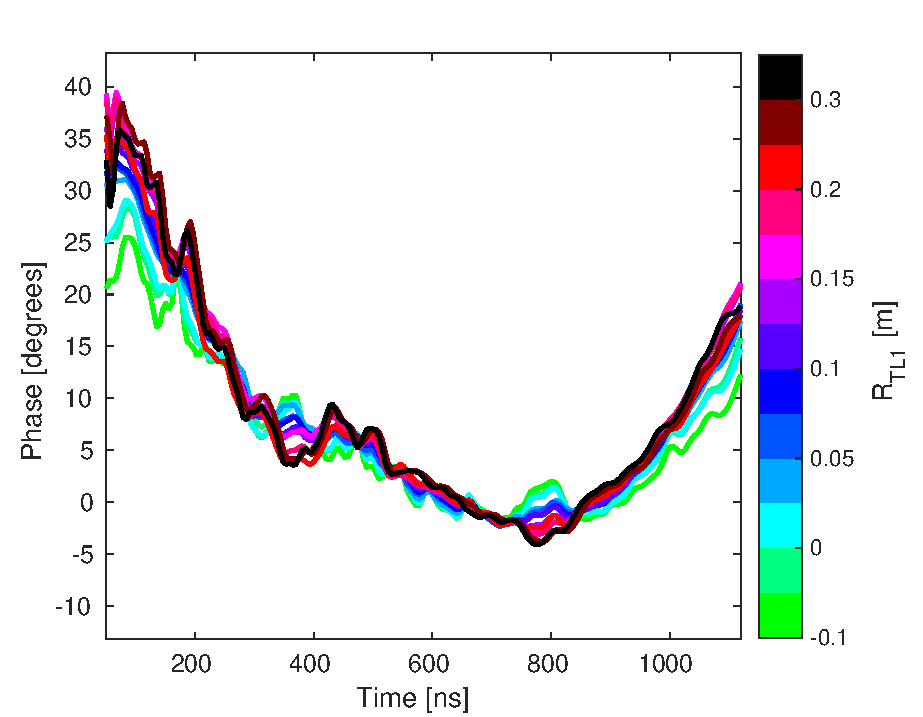
\includegraphics[width=0.9\textwidth]{Figures/propagation/r56Scan_meanPhaseAlong}
  \caption{Mean downstream phase along the pulse for different R56 values.}
  \label{f:r56Scan_meanPhaseAlong}
\end{figure}

The difference between the phase along the pulse for two different settings of R56 in TL1 should be proportional to the beam energy along the pulse. Figure~\ref{f:r56Scan_comparisonPhaseEnergy} plots the difference between the R56~=~+0.3~m optics and the optimal R56~=~+0.175~m optics, and compares this to the beam energy along the pulse (measured using the horizontal beam position in the dispersive BPM after the first dipole in TL1). Both lines are mean subtracted and normalised to give equivalent amplitudes in arbitrary units. For reference the peak to peak beam position offset along the pulse is 1.6~mm in this case, coresponding to a relative energy offset along the pulse of \(2.3\times10^{-3}\). Overall, the differences in phase along the pulse resulting from using non-optimal R56 in TL1 are very well matched with the energy variation along the pulse, as expected.

\begin{figure}
  \centering
  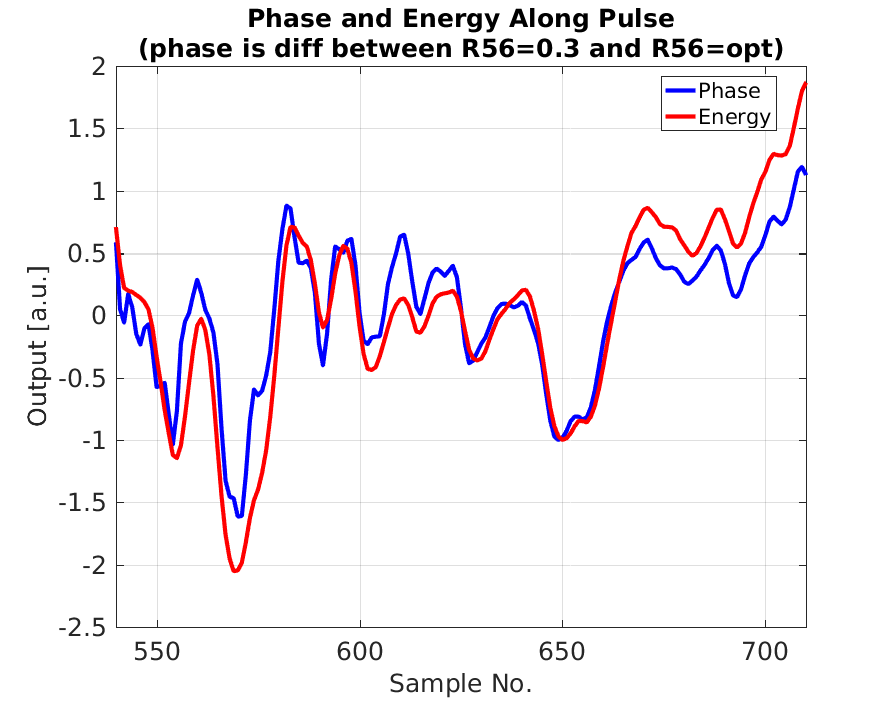
\includegraphics[width=0.9\textwidth]{Figures/propagation/r56Scan_comparisonPhaseEnergy}
  \caption{Mean downstream phase along the pulse for different R56 values.}
  \label{f:r56Scan_comparisonPhaseEnergy}
\end{figure}

[TODO: comparison of upstream and downstream phase along the pulse]

[TODO: Jitter along the pulse]

\subsubsection{Results from Other Scans}

\newsection{t566}{Higher Order Energy Dependencies}

\subsection{Expected Dependence due to Optics}
\label{ss:t566Sim}

\subsection{Energy Variation Along the Pulse}
\label{ss:energyAlongPulse}

and different R56 optimal point along pulse

\subsection{R56 Scans whilst Varying Beam Energy}
\label{ss:r56ScanWithEnergy}

\begin{figure}
  \centering
  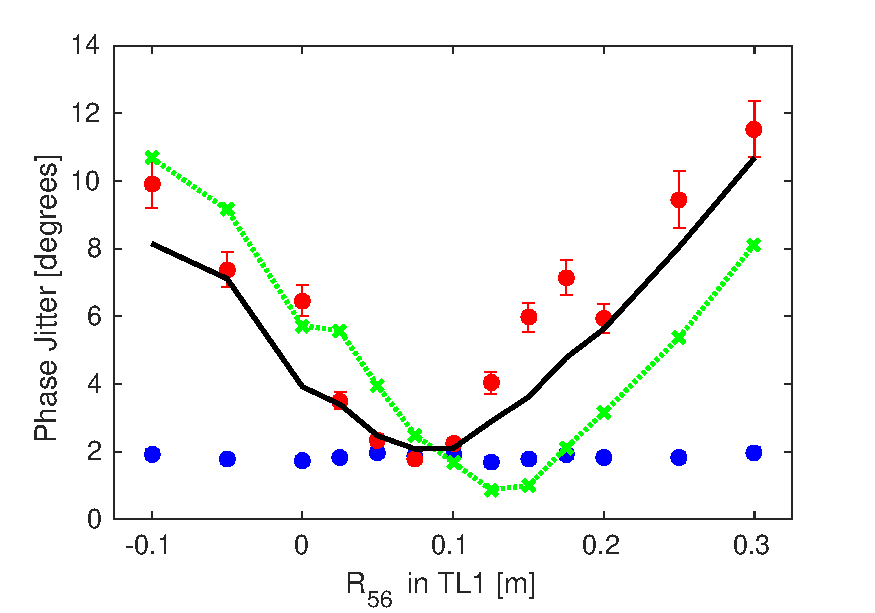
\includegraphics[width=0.9\textwidth]{Figures/propagation/R56ScanGunWiggle_PhaseJitter}
  \caption{Phase jitter for different R56 whilst wiggling gun current.}
  \label{f:R56ScanGunWiggle_PhaseJitter}
\end{figure}

\begin{figure}
  \centering
  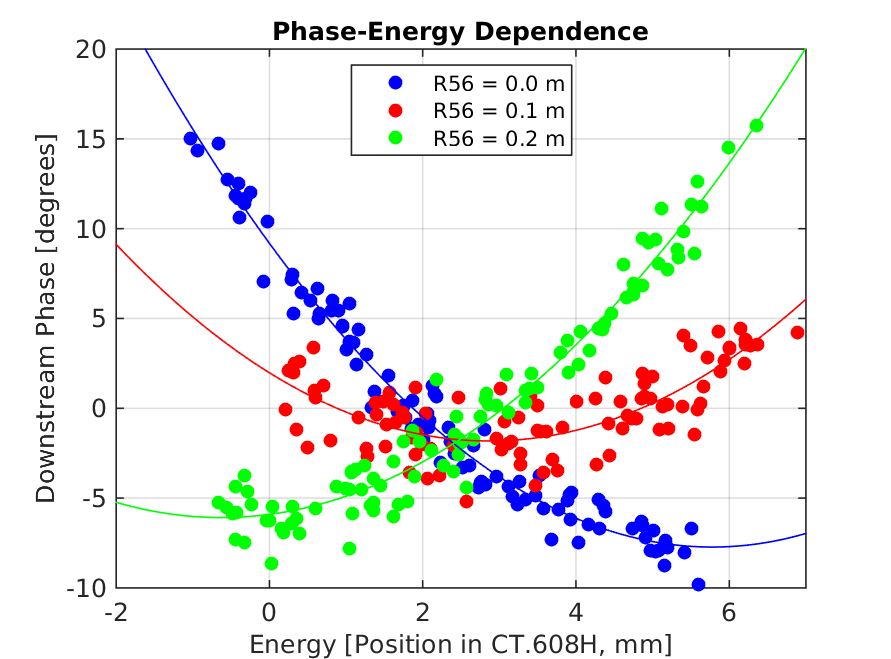
\includegraphics[width=0.9\textwidth]{Figures/propagation/R56ScanGunWiggle_Vs608}
  \caption{Phase vs. energy for different R56 in TL1.}
  \label{f:R56ScanGunWiggle_Vs608}
\end{figure}

\subsection{Mitigation of Higher Order Dependencies}
\label{ss:t566Mitigation}



\subsection{Effect on PFF Operation}
\label{ss:t566EffectPFF}


\newsection{otherJitterSources}{Other Sources of Phase Jitter}

\subsection{Combiner Ring Septum}
\label{ss:crSeptum}

\subsection{TL1 \& Combiner Ring Bends}
\label{ss:crBends}


RF Deflector

CR Septum

TL1/CR Bends


\newsection{bestPhaseProp}{Best Phase Propagation}

some kind of drift analysis of drift sources to be able to refer back to it in long PFF results section



